\documentclass[final,hyperref={pdfpagelabels=false}]{beamer}
\mode<presentation>
  {
   %\usetheme{Berlin}
  \usetheme{Dreuw}
  }
  %\usepackage{times}
  \usepackage{amsmath,amsthm, amssymb, latexsym}
  \boldmath
  \usepackage[english]{babel}
  \usepackage[latin1]{inputenc}
  \usepackage[orientation=landscape,size=a0,scale=1.4,debug]{beamerposter}
  \usepackage{epstopdf}
  \usepackage{subcaption}

  \usepackage{tikz}
\usetikzlibrary{shapes,arrows}
  %%%%%%%%%%%%%%%%%%%%%%%%%%%%%%%%%%%%%%%%%%%%%%%%%%%%%%%%%%%%%%%%%%%%%%%%%%%%%%%%%
  \graphicspath{{figures/}}
  \title[NNV]{Neural Network Visualization}
  \author{Zijian Li, Callin Switzer, Yue Zhao and Zhengde Zhao}
  \vspace{5cm}
  \institute{University of Washington}
  \date{June 10th, 2019}
	 	
\usefonttheme[onlymath]{serif}


  %%%%%%%%%%%%%%%%%%%%%%%%%%%%%%%%%%%%%%%%%%%%%%%%%%%%%%%%%%%%%%%%%%%%%%%%%%%%%%%%% 
\begin{document}

  \begin{frame}{}

    \begin{columns}[t]
      \begin{column}{.32\linewidth}
        \begin{block}{Motivation}
 \noindent       Learning a non-linear controller for insect flight dynamics with a deep neural network
 \begin{center}
          \includegraphics[scale=0.9]{s1.pdf}
  \end{center}         
\noindent        \textbf{ Question}: What is the temporal pattern of forces required to follow a complex trajectory?  If I know where I am, and where I want to go, how do I get there?
\begin{center}
          \includegraphics[scale=1]{s3.pdf}
\end{center}
\noindent   \textbf{ Answer}: Deep learning + Model Predictive Control 
\begin{center}
\includegraphics[scale=0.9]{s2.pdf}
\end{center}         
\noindent       \textbf{ Goal}:   Visualize the "internal workings" of a feed forward neural network.        
   \end{block}

    \vfill
   \end{column}

      \begin{column}{.4\linewidth}
      \begin{block}{Visualizing neural network architecture}
      \noindent This is a nerual network with $3$ hidden layers of size: $20,\ 20,\ 16$.\\
      \noindent The inputs are: $\phi_0=\theta_0=\dot{x}_0=\dot{y}_0=\dot{\phi}_0=\dot{\theta}_0=-0.5$ and  $x_f=y_f=\phi_f=\theta_f=0.5$.
      \vspace{3cm}
      \begin{center}
                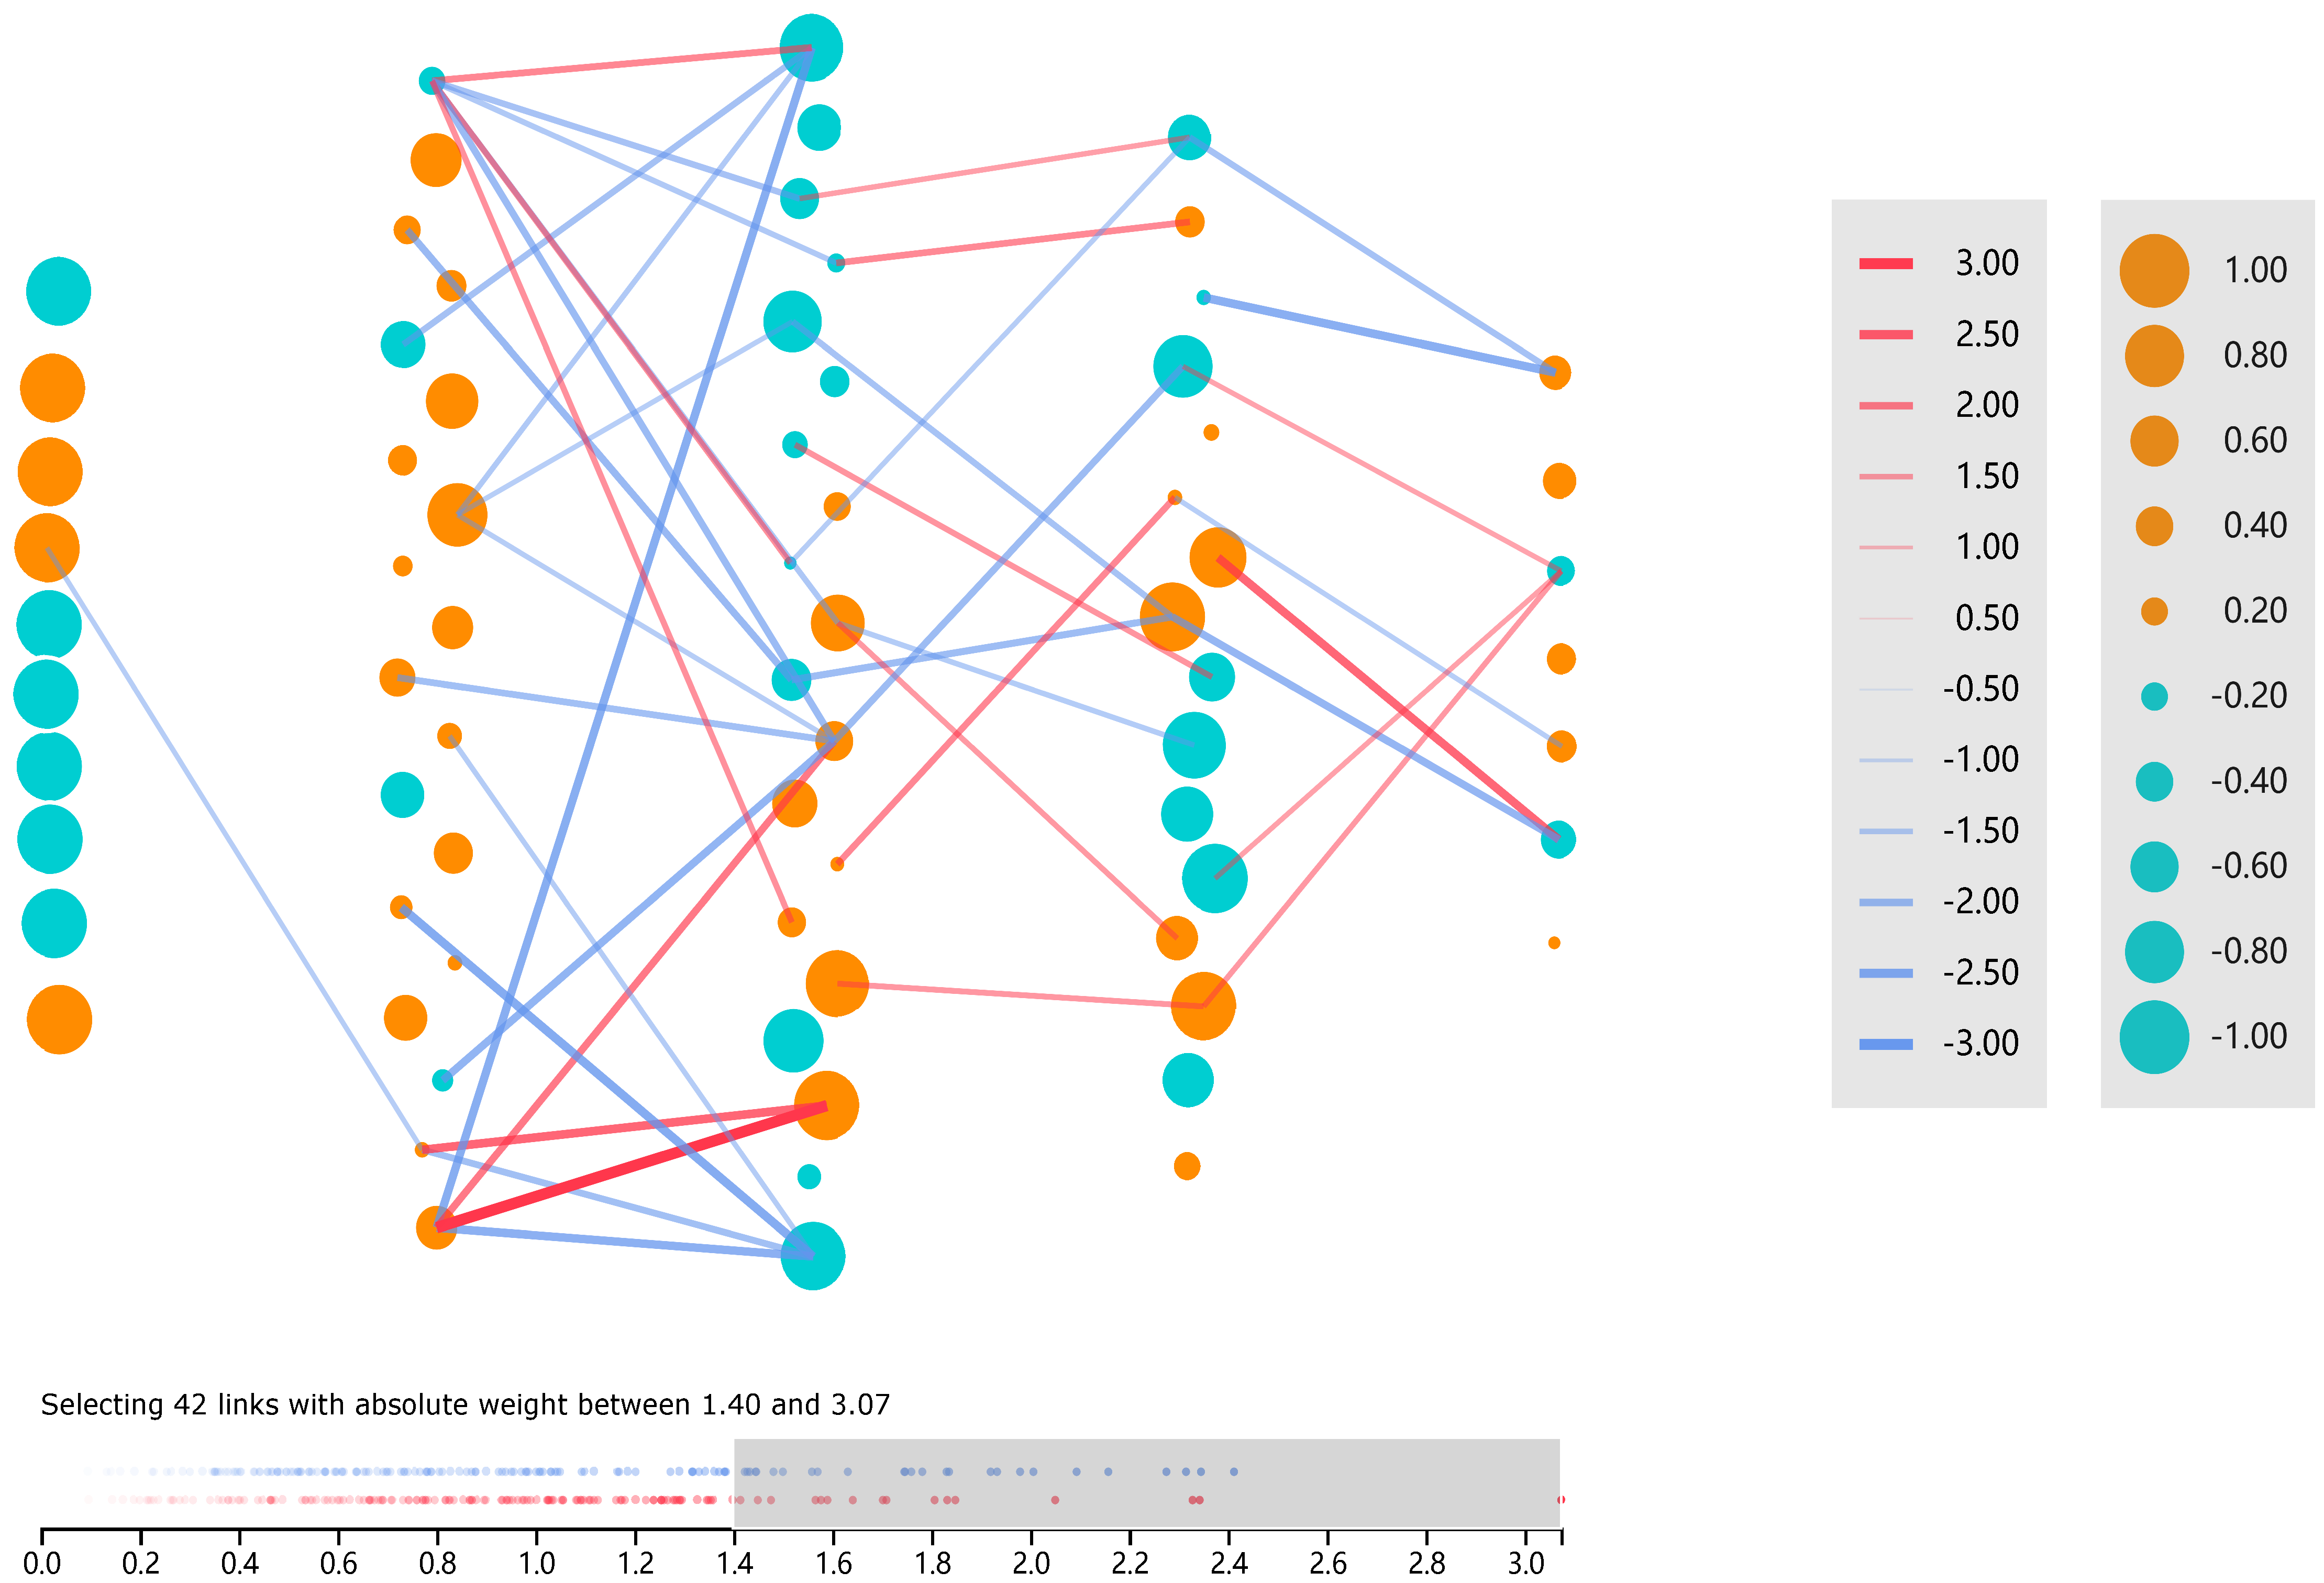
\includegraphics[scale=0.5]{chart1.eps}
      \end{center}
      \vspace{4cm}
        \noindent This is a nerual network with $4$ hidden layers of size: $512,\ 512,\ 512,\ 512$.\\
      \noindent The inputs are: $\phi_0=\theta_0=\dot{x}_0=\dot{y}_0=\dot{\phi}_0=\dot{\theta}_0=x_f=y_f=\phi_f=\theta_f=0$.
       \vspace{3cm}
       \begin{center}
                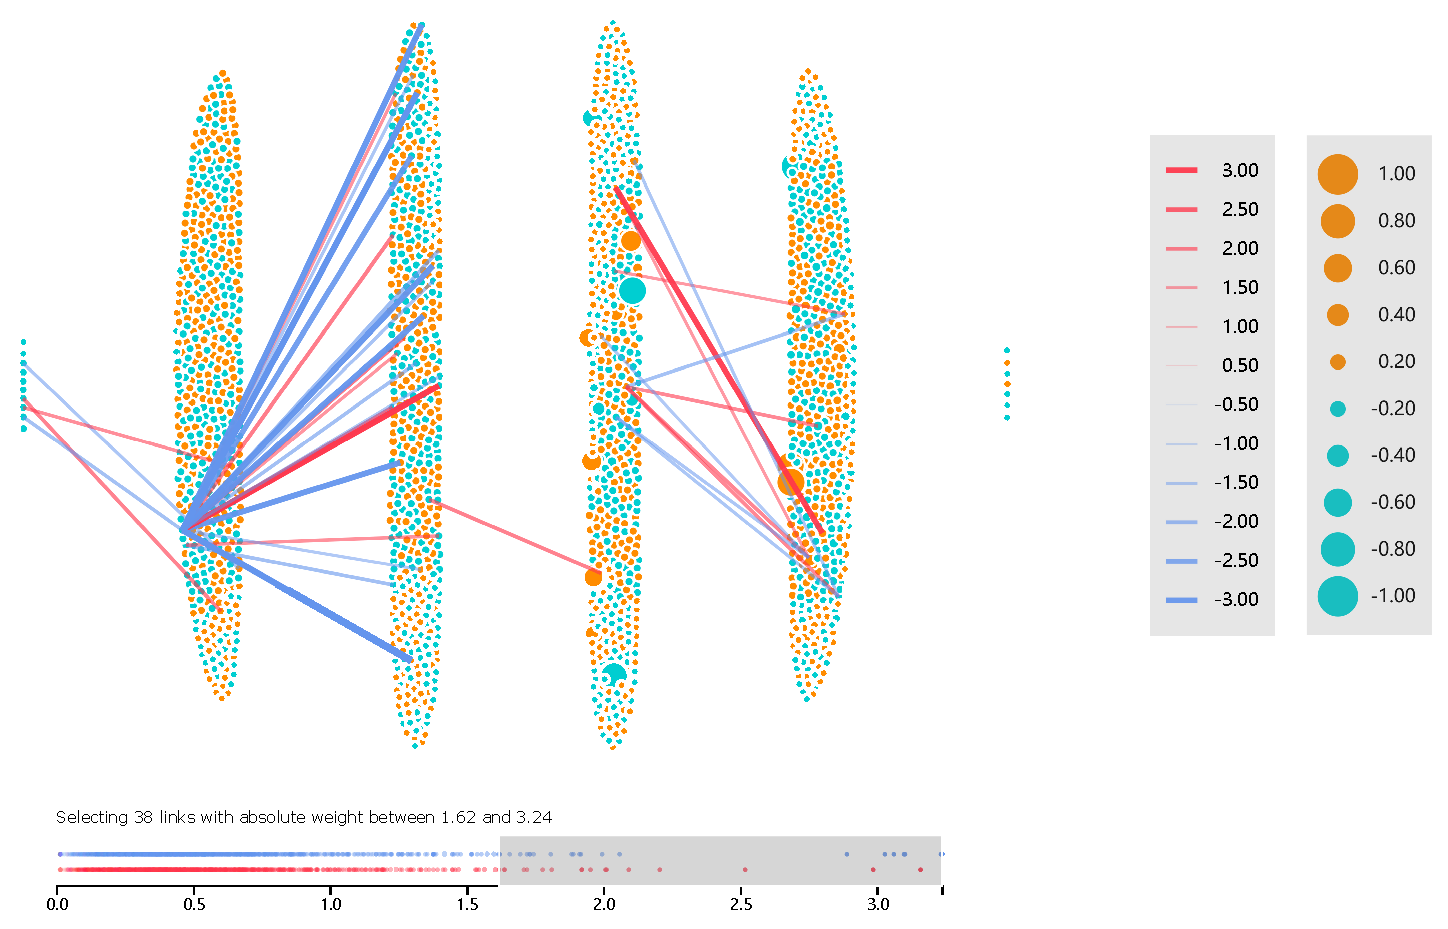
\includegraphics[scale=1.5]{chart3.eps}
      \end{center}
      \vspace{3cm}
      \end{block}
      \end{column}
\begin{column}{.25\linewidth}
\begin{block}{Interaction techniques}
\begin{itemize}
\item The nodes can be dragged to re-position.
\item Dropdown menu that allows to choose different neural network.
\item Sliders that allow to choose values for each input variable.
\item The brush allows to choose the range of the weight (in absolute value) to be shown.
\item When hover on the nodes or links, the details will show up.
\end{itemize}
\end{block}    
\begin{block}{Improvements}
\begin{itemize}
\item Hide all ``dead'' nodes
\item For any node, show the strongest path.
\end{itemize}
\end{block}   

      
      \end{column}

      
    \end{columns}
  \end{frame}
\end{document}


%%%%%%%%%%%%%%%%%%%%%%%%%%%%%%%%%%%%%%%%%%%%%%%%%%%%%%%%%%%%%%%%%%%%%%%%%%%%%%%%%%%%%%%%%%%%%%%%%%%%
%%% Local Variables:
%%% mode: latex
%%% TeX-PDF-mode: t
%%% End:
